\chapter{Theoretical analysis of the~KSA}
\TODO{je to po popisu utoku, takze to chce rict, ktery resim } 

This thesis is focused to deriving the secret key from the inner state after KSA. The permutation after the KSA algorithm is biased towards the secret key. Class of key retrieval algorithms which uses the inner state can benefit from that fact to extract complete key or information about some of its bytes. 

There are two types in biases The most likely value y-th element of permutation after complete KSA is
\TODO{In 1995 Roos observed, that 2}\\


\[ S_{N}[y] = \dfrac{y(y+1)}{2} + \K{0}{y}\]

 This equation has high probability on \TODO{formulace} first $ \sim 40 $ entries is

 It is because with hight probability happens event \TODO{event} described bellow. Similarly with last $ \sim 40 $ entries and inverse permutation. 

We can also use the fact, that with certain probability values of indices $ j_{i} $ can be found in the inner permutation or the inverse permutation and using the update rule

\[ j_{i+1} = j_{i} + S[i] + K[i\Mod{l}] \].


\TODO{Roos in 1995 } 

%[6] noticed that some of the elements of the initial permutations have a
%bias towards a linear combination of the secret key bytes. A theoretical proof of these
%biases was given by Paul and Maitra [5], later generalized by Biham and Carmeli [2].
%Thanks to our choice C[−1] = 0, these results can be given in a unified theorem as
%	follows.

Most likely value of , denoted $ S_{N}[y] $, is given by 
\[ S_{N}[y] = \dfrac{y(y+1)}{2} + \K{0}{y} \]


Hlavni myslenka, nektere klice jsou pravdepodobnejsi nez jine, z toho vnitrniho stavu!! 

We will use both facts in the key retrieval algorithm.



%%%%%%%%%%% Probability introduction %%%%%%%%%%%%
%%%%%%%%%%%%%%%%%%%%%%%%%%%%%%%%%%%%%%%%%%%%%%%%%

%%%%%%%%%%% Probability introduction %%%%%%%%%%%%
%%%%%%%%%%%%%%%%%%%%%%%%%%%%%%%%%%%%%%%%%%%%%%%%%

\chapter{Preliminaries}

\TODO{kapitolu dodelat pozdeji}
\TODO{k tomuto nejaky uvod?}
\begin{defn}
	A \defined{discrete probability space} is a pair
	$ (\Omega,\Pr) $ consisting of:
	
	\begin{enumerate}
	\item A nonempty countably infinite set $ \Omega $.
	\item A function $ \Pr: \Omega \rightarrow R $, called probability measure, 
	satisfying the following properties:
		\begin{enumerate}
			\item $  \forall \omega \in \Omega: 0 \leq Pr(\omega) \leq 1 $ %% positivity
			\item $ \sum_{\omega \in \Omega}\Pr({\omega}) = 1 $.
		\end{enumerate}
	\end{enumerate}
\end{defn}

\begin{defn}
	Let $ (\Omega,\Pr) $ be a discrete probability space. An \defined{event} $ E $ is any finite subset of $ \Omega $. The probability of $ E $ is defined as 
	$ \Pr(E) = \sum_{\omega \in E}\Pr(\omega)  $ and $ \Pr(\emptyset) = 0$.
\end{defn}

\begin{defn}
	Let $ (\Omega, \Pr) $ be a discrete probability space and $ E_{1}, E_{2} \subseteq \Omega $  where $ E_{2} \neq 0 $. Then we define \defined{conditional probability} as follows:
	
	 \[ Pr(E_{1} | E_{2}) = \dfrac{\Pr(E_{1} \cap E_{2})}{\Pr(E_{2})} \]
\end{defn}

\begin{lemma}
	\TODO{zakladni vztahy}
	\[ \Pr(A \cup B) = \Pr(A) + \Pr(B) - \Pr(A \cap B) \]
	\[\Pr(\complem{A}) = 1-\Pr(A)\]
\end{lemma}


\begin{thm}
	(The law of total probability)
	
	\begin{equation}\label{totalProb}
	\Pr(E) = \sum_{n}\Pr(A \cap B_{n}) = \sum_{n}\Pr(A \, | \, B_{n})\Pr(B_{n})
	\end{equation}
	
	
	
	\TODO{veta o uplne pravdepodobnosti}
\end{thm}

\begin{defn}
	\TODO{\textbf{Uniform distributio}n takto nebo musim zavadet jevy jako zobrazeni?}
	$ \forall \omega \in \Omega : \Pr(\omega) = \dfrac{1}{|\Omega|} $
\end{defn}

\begin{defn}
Two events $ A $ and $ B $ are independent (often written as $ A \perp B  $) if and only if their joint probability equals the product of their probabilities:

\[ \Pr{(A \cap B)} = \Pr{(A)}\Pr{(B)}. \]
\end{defn} 

\begin{notation}
		\red{$ \complem{A} $ is complementary event to $ A $}
\end{notation}
	



%%%%%%%%%%% Notations                %%%%%%%%%%%%
%%%%%%%%%%%%%%%%%%%%%%%%%%%%%%%%%%%%%%%%%%%%%%%%%
\section{Notations and basic assumptions}

\begin{notation}
	Let $ K $ be the array of key bytes \red{with} length $ l $. We will \red{denote} 
	
	\[\K{a}{b} \coloneqq \sum\limits_{i=a}^{b}K[i \Mod{l}] 	\]
	
	The indice $ j $ in $ r $-th round of the KSA will be noted $ j_{r} $, the permutation after $ r $ rounds will be $ S_{r} $. Therefore $ S_{N} $ is the permutation after complete KSA.
	
	$ 	\InvS $ will stand for the inverse of the permutation $ S $, i.e. $ \forall y \in \FromTo{0}{N-1}: S[y] = v \Rightarrow \InvS[v] = y$.
	

	\red{Mozna jeste $ K[a] = K[a \Mod{l}] $}
\end{notation}


%%%%%%%%%%% Prvni bias %%%%%%%%%%%%%%%%%%%%%%%%%%
%%%%%%%%%%%%%%%%%%%%%%%%%%%%%%%%%%%%%%%%%%%%%%%%%

\section{Roos bias}


	%%% Prerekvizita vety 
	\begin{lemma}
		\red{prerekvizita vety 1}
		Assume that the index $ j $ takes its value from $ \Z_{N}  $ uniformly at random at each round of the KSA. Then $ \forall y \in \Z_{N} $:
		
		\[ \Pr\Big(j_{y+1} = \dfrac{y(y+1)}{2} + \K{0}{y} \Big) 
		\approx 
		\Big(\dfrac{N-1}{N}\Big)^{1+\frac{y(y+1)}{2}} + \dfrac{1}{N}
		\]
		
	\end{lemma}		
	\begin{proof}
		Let $ E_{y} $ denote the event that $ j_{y+1} = \sum_{x=0}^{y}(y + K[x mod l])$
	\end{proof}	
	
	%%% Prerekvizita vety 	
	\begin{lemma}
		\TODO{prerekvizita vety 1}
	\end{lemma}



	
	\begin{thm}{\cite{GoMa}}
		Assume that during the KSA the index j takes its values uniformly at random from $ \Z_{N} $. Then $ \forall 0 \leq i \leq r-1, 1 \leq r \leq N $
		
		\[ \Pr(S_{r}[i] = \K{0}{i} + \dfrac{i(i+1)}{2})   \geq (\dfrac{N - i}{N})(\dfrac{N-1}{1})^{\frac{i(i+1)}{2}+r}+\dfrac{1}{N} \]
	\end{thm}
	
	\begin{proof}
		\TODO{dukaz}
	\end{proof}
	
	\begin{cor}
	\TODO{zobecneni na posledni kolo nebo predchozi vetu rovnou smerovat tam?}
\end{cor}
	
\TODO{tabulka s aktualnimi hodnotami } 

\TODO{to same pro InvS} 


\begin{thm}
	After the complete KSA, 
	\[  \Pr(S_{N}[S_{N}[y]] = \K{0}{i} + \dfrac{i(i+1)}{2}) \approx  \]
	
	clanek 4, appendix, na zacatku graf
\end{thm}

\TODO{tabulka s aktualnimi hodnotami, dukaz}


\begin{notation}
		\[  C_{y} = S_{N}[y] - \dfrac{y(y+1)}{2} \]
\end{notation}

\TODO{zobecneni na sekvence}


\TODO{inverzni sekvence}

\TODO{vyyiti tohoto na ziskani klice - rovnice} 


\section{Substracting equations}

Let $i_{1} < i_{2} $. If $ C_{i_{1}} = \K{0}{i_{1}} $ and $ C_{i_{2}} = \K{0}{i_{2}} $, then we can substract the values and get
\[ C_{i_{2}} - C_{i_{1}} = \K{0}{i_{2}} - \K{0}{i_{1}} = \K{i_{1} + 1}{i_{2}}	\].

This holds with the product of the individual probabilities of $ C_{i} $



%%%%%%%%%%% Druhy bias               %%%%%%%%%%%%
%%%%%%%%%%%%%%%%%%%%%%%%%%%%%%%%%%%%%%%%%%%%%%%%%
\section{Useful distributions for The Key Recovering Algorithm}

\begin{defn}
If $ j_{i} = S[i] $, we call this as event 1 has occured for index $ i $, and denote as $ E_{1} $.
\end{defn}

\begin{thm}
\[	P(S[i] = j_{i}) \geq (1-\dfrac{1}{N})^{i}(1-\dfrac{i-1}{N})(1-\dfrac{1}{N})^{N-i-1}+ \dfrac{1}{N} \]
\end{thm}

\begin{defn}
	If $ j_{i} = S[i] $, we call this as event 1' has occured for index $ i $, and denote as $ E'_{1} $.
\end{defn}

\begin{thm}
	\[	P(S^{-1}[i] = j_{i}) \geq (\dfrac{i}{N})(1-\dfrac{1}{N})^{N-1}+ \dfrac{1}{N}\]
\end{thm}


\begin{proof}
		$ (1-\dfrac{1}{N})^{i}(\dfrac{i}{N})(1-\dfrac{1}{N})^{N-i-1}+ \dfrac{1}{N} $
\end{proof}

\begin{thm}
	$ P(S[i] = j_{i} \vee S^{-1}[i] = j_{i}) $ used for BuildKeyTable algorithm in paper 1
\end{thm}


\TODO{ $ P(S[S[i]] = j_{i}) $ - dukazy nikde nejsou...}

\TODO{ $ P(S^{-1}[S^{-1}[i]] = j_{i}) $}

\TODO{ $ P(S[S[S[i]] = j_{i}) $}

\begin{figure}
\centering
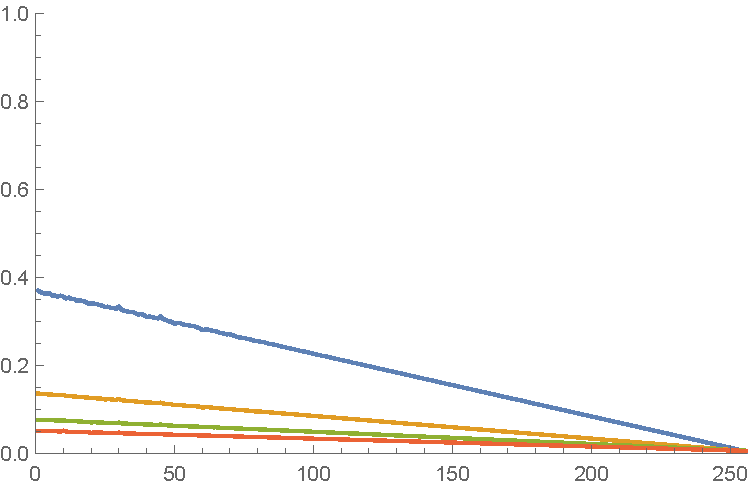
\includegraphics[width=0.7\linewidth]{img/all}
\caption[All]{hallo}
\label{fig:all}
\end{figure}


\TODO{experimentalne... rychle to konverguje}



